\documentclass[cs4size,a4paper,nofonts]{ctexart}
\usepackage[utf8]{inputenc}
\def\tjf{{\tt{田劲锋}}}
\def\titlec{用哈夫曼算法压缩文件}
\def\titlee{File~Compression with Huffman~Algorithm}
\usepackage[top=2.5cm,bottom=2.5cm,left=3.1cm,right=3.1cm]{geometry} % 页面设置
\usepackage[unicode,breaklinks=true,
colorlinks=true,linkcolor=black,anchorcolor=black,citecolor=black,urlcolor=black,
pdftitle={\titlec},pdfauthor={\tjf},pdfsubject={\titlee}]{hyperref}
\usepackage{tikz} % 画图
\usetikzlibrary{shapes,arrows}
\usepackage{multicol} % 分栏
\usepackage{multirow} % 跨行
\usepackage{longtable} % 长表格
\usepackage{tabularx} % 变宽表格
\usepackage{booktabs} % 表格画线
\usepackage{graphicx} % 图形
\usepackage{color} % 颜色
\usepackage{xcolor} % 颜色
\usepackage{wallpaper} % 背景图片
\usepackage{listings} % 排版代码
\usepackage{verbatim} % 排版代码
\usepackage{url} % 排版链接
\usepackage{shortvrb}
\usepackage{pstricks} % 绘图
\usepackage{pst-tree} % 画树
% \usepackage{pst-uml} % 画 UML
\usepackage{uml} % 画 UML
\usepackage{clrscode3e} % CLRS 伪代码
\usepackage{smartdiagram} % 智能画图
\usepackage{nameref}
\usepackage{rotating} % 横排大图
\usepackage{caption}
\captionsetup{font={small}} % 标题字体大小
\usepackage[inline]{enumitem} % 调整列表样式

\setmainfont{Times New Roman}
\setCJKmainfont[BoldFont={SimHei}]{SimSun}  % 主要字体:宋体、黑体
\setCJKsansfont[BoldFont={STZhongsong}]{STFangsong} % 次要字体:仿宋、中宋
\setCJKmonofont{KFKai} % 等宽字体:楷体
\setCJKfamilyfont{msyh}[BoldFont={* Bold}]{微软雅黑} \newcommand{\msyh}{\CJKfamily{msyh}} % 微软雅黑
\setCJKfamilyfont{micro}{文泉驿微米黑} \newcommand{\micro}{\CJKfamily{micro}} % 文泉驿微米黑
\setCJKfamilyfont{liti}{隶书} \newcommand{\liti}{\CJKfamily{liti}}

\CJKsetecglue{\hspace{0.1em}}
\renewcommand\CJKglue{\hskip -0.3pt plus 0.08\baselineskip}
\frenchspacing
\widowpenalty=10000
\linespread{1.5} % 1.5 倍行距
\setlength{\parskip}{2pt plus 2pt}
\renewcommand{\baselinestretch}{1.5}

\setlength{\abovecaptionskip}{1pt}
\setlength{\belowcaptionskip}{0pt}
\setlength{\intextsep}{8pt}

\makeindex
\pagestyle{plain}

\begin{document}
\newcommand{\tabincell}[2]{\begin{tabular}{@{}#1@{}}#2\end{tabular}}
\newcommand{\tabincelll}[3]{\begin{tabular*}{#1}{@{}#2@{}}#3\end{tabular*}}
\renewcommand{\tabularxcolumn}[1]{m{#1}}
\newcommand{\vil}{\,\vline \hspace{.5em} }


\newcommand{\des}[2]{\makebox[2em][s]{\bf #1}\quad #2}
\newcommand{\function}[5]{\CTEXnoindent\vspace{1em}\par
\begin{minipage}{\textwidth}
    \underline{\makebox[\textwidth][l]{\it{#1}}}\\
    {\tt {{#3}} {\bfseries #1}(#2);}\\
    \des{返回}{#4}\\
    \des{描述}{#5}
\end{minipage}\par
\CTEXindent}

\newcommand\pictext{\linespread{1}\centering}

\lstset{language=C++,
  numbers=left,
  keywordstyle=\bfseries,
  frame=tb,
  morekeywords=[1]{perror,assert,printf,fprintf,scanf,sscanf},
  morekeywords=[2]{},
}


%%%% 开始 %%%%
\begin{titlepage}

\begin{center}


\includegraphics[height=1cm]{image/haut.png}

\vspace*{1cm}
{\liti\fontsize{48pt}{50pt}{课\quad 程\quad 设\quad 计}}

\vspace*{4cm}
{\fontsize{36}{80}\sf\bfseries \titlec}

\vspace*{1cm}
{\fontsize{30}{70}\sf\bfseries \titlee}

\vfill
{\large
\newcommand{\ctline}[2]{\makebox[6em][s]{\bf #1}:\underline{\makebox[14em][c]{\qquad #2\qquad}}\\}
\ctline{课程设计名称}{数据结构课程设计}
\ctline{专业班级}{计算机 1303 班}
\ctline{学生姓名}{\tjf}
\ctline{学号}{201316920311}
\ctline{指导教师}{白\quad 浩}
\ctline{课程设计时间}{\today}
}

\end{center}

\end{titlepage}
\newpage
\pagestyle{empty}\quad\newpage
\section*{\underline{~软件工程~}专业课程设计任务书}
% \addcontentsline{toc}{section}{课程设计任务书}
% \ThisCenterWallPaper{1}{source/task.pdf}
\begin{center}

\begin{tabular}{|c|c|}\hline
{\bf 学生姓名} & \makebox[5em][c]{\tjf} \vil
\makebox[4em][c]{\bf 专业班级} \vil
\quad 软件 1305 班 \quad \vil
\makebox[4em][c]{\bf 学~号} \vil
201316920311 \\\hline
{\bf 题~目} & \quad \titlec \\\hline
{\bf 课题性质} & \makebox[12em][c]{其他} \vil
{\bf 课题来源} \vil \makebox[11em][c]{自拟课题} \\\hline
{\bf 指导教师} & \makebox[12em][c]{刘扬} \vil
{\bf 同组姓名} \vil \makebox[11em][c]{无} \\\hline
{\bf 主要内容} & {\begin{minipage}[c][5cm][c]{12cm}
操作系统是控制应用程序执行的程序,并充当应用程序和计算机硬件之间的接口。一个操作系统的主要功能有:
\begin{enumerate}
\item 处理器管理
\item 存储器管理
\item 设备管理
\item 文件管理
\end{enumerate}
现在的桌面操作系统多是多任务分时操作系统。
\end{minipage}} \\\hline
{\bf 任务要求} & {\begin{minipage}[c][5cm][c]{12cm}
目标是完成一个基本可用的图形界面操作系统,包括如下基本模块:
\begin{enumerate}
\item 进程:中断处理、多任务调度、系统保护
\item 存储管理:内存分配、进程空间管理
\item I/O 系统:鼠标、键盘和屏幕的控制
\item 文件系统:文件与可执行程序的读取和加载
\end{enumerate}

系统提供命令行用户接口和图形化用户接口,允许使用 C 语言编写系统应用程序,可以从 FAT12 格式软盘启动。
\end{minipage}} \\\hline
{\bf 参考文献} & {\begin{minipage}[c][5cm][c]{12cm}
川合秀实. 30天自制操作系统. 人民邮电出版社, 2012\\
W. Stallings. 操作系统: 精髓与设计原理(第6版). 机械工业出版社, 2010\\
R. E. Bryant, 等. 深入理解计算机系统系统(第2版). 机械工业出版社, 2010\\
A.S.Tanenbaum, 等. 操作系统设计与实现. 电子工业出版社, 2007\\
W. R. Stevens, 等. UNIX环境高级编程(第3版). 人民邮电出版社, 2014
\end{minipage}} \\\hline
{\bf 审查意见} & {\begin{minipage}[c][5cm][c]{12cm}
    指导教师签字:\\
    \vspace*{2cm}\\
    教研室主任签字:\hspace{6cm} 2015~年~6~月~25~日
\end{minipage}} \\\hline
\end{tabular}

\small 说明:本表由指导教师填写,由教研室主任审核后下达给选题学生,装订在设计(论文)首页

\end{center}
\quad\newpage
\setcounter{page}{0}\pagestyle{plain}
\linespread{1}\tableofcontents\linespread{1.5}\newpage
\section{需求分析}

\subsection{任务探究}

大一最后的课程——程序设计实践,目的是加深对 C 语言的理解和使用,为后来的学习打好基础。课程设计要求做一个标准化考试系统。

% 任务书要求如下:
% \begin{quote}\small
% \tasktext
% \end{quote}

考虑基本功能,即是对题目数据库的增、删、改、查(用文件存取数据),以及按一定策略生成试卷。

考虑扩展功能,需要实现用户模块和权限处理,还有简单的成绩管理。

\subsection{界面模块}

对于本程序而言,我们不需要复杂的 GUI(图形用户界面)。因为标准 C 中并没有直接对图形操作的库,直接调用 Windows API 会无法移植到类 UNIX 操作系统,并且程序会相当复杂。如果可能的话,我更喜欢用 Web 的方式呈现,当然这也需要使用相应的编程工具链,不是标准 C 可以简单做到的。

所以我决定采用纯文本命令行界面,如非必要不对终端界面进行特殊设置。本来是要实现命令行参数接口的,限于时间关系,未能完成。目前的界面只是简单地文本状态下的用户交互,提供简单的容错处理。

考虑用户界面,提供学生和教师两个入口。如图~\ref{al_main}~所示,主界面提供了两个用户入口,并提供了帮助和关于。

\begin{figure}[htp]
\pictext
% \begin{tikzpicture}[align=center](10,4)
% % \draw[help lines] (0,0) grid (10,3);
% \node (main) at (5,4) [draw] {入口主界面};
%   \node (student) at (2,2) [draw] {学\\生\\登\\录};
%   \draw[-] (student) |- (5,3.3) -| (main);
%   \node (teacher) at (4,2) [draw] {教\\师\\登\\录};
%   \draw[-] (teacher) |- (5,3.3) -| (main);
%   \node (help) at (6,2) [draw] {帮\\助};
%   \draw[-] (help) |- (5,3.3) -| (main);
%   \node (about) at (8,2) [draw] {关\\于};
%   \draw[-] (about) |- (5,3.3) -| (main);
% \end{tikzpicture}
\smartdiagram[bubble diagram]{主界面,
帮助,
学生\\登录,
关于,
教师\\登录
}
\caption{\label{al_main}主要模块}  
\end{figure}

\subsubsection{学生功能模块}

学生模块属于扩展功能,如图~\ref{al_student}~,提供做卷子和看成绩两个模块入口。

\begin{figure}[htp]
\pictext
\smartdiagram[constellation diagram]{学生\\主界面,
做卷子,
看成绩
}
\caption{\label{al_student}学生功能模块}  
\end{figure}

\subsubsection{教师功能模块}

教师模块是本程序的主要部分。如图~\ref{al_teacher}~所示,应该实现试题的增、删、改、查功能,实现一定策略的“智能”组卷算法。作为扩展功能,实现对成绩的查看。

\begin{figure}[htp]
\pictext
\smartdiagram[constellation diagram]{教师\\主界面,
浏览\\试题,
添加\\试题\\(增),
删除\\试题\\(删),
修改\\试题\\(改),
查询\\试题\\(查),
智能\\组卷,
成绩\\分析
}
\caption{\label{al_teacher}教师功能模块}  
\end{figure}

目前不需要做到批量增、删、改,其对象是应当是唯一的,这里我们用题目编号来指定。

对于查询操作,应该提供多种方式。如图~\ref{al_select}~,可以根据试题某个属性单独查询,也应提供模糊查询以查询所有选项。

\begin{figure}[htp]
\pictext
\smartdiagram[constellation diagram]{查询\\试题,
编号,
描述,
选项,
难度,
标签,
章节,
模糊\\查询
}
\caption{\label{al_select}试题查询模块}  
\end{figure}

对于组卷功能,我们应该提供多种算法。如图~\ref{al_generate}~,可以完全随机生成,也可以指定标签、章节、难度对试卷进行生成。另外,这里也可以查看已生成试卷列表和内容。

\begin{figure}[htp]
\pictext
\smartdiagram[constellation diagram]{智能\\组卷,
随机\\生成,
按标签\\生成,
按章节\\生成,
按难度\\生成,
试卷\\列表,
查看\\试卷
}
\caption{\label{al_generate}试卷模块}  
\end{figure}

\section{概要设计}

% \subsection{函数调用关系}

\begin{sidewaysfigure}
\centering
\newcommand{\defun}[2]{{\it #2}\\ {#1}}
% \newcommand{\defun}[2]{{#1}}

% \smartdiagram[constellation diagram]{
% \defun{编码文件}{huffman encode file},
% \smartdiagram[sequence diagram]{
%   \defun{获取频率}{get symfreq},
%   \defun{新叶结点}{new leaf node},
%   \defun{建立符号编码表}{build symcode},
%   },
% \defun{计算编码}{calc code},
% \defun{写出编码表}{write code table},
% \defun{编码}{do file encode},
% \defun{销毁编码表}{free encoder},
% \defun{销毁树}{free tree}
% }
\begin{tikzpicture}[align=center]
% \draw[help lines] (0,0) grid (20,11);

\node (A) at (27em,10) [ellipse,draw] {\defun{压缩文件}{huffman\_encode\_file}};
  \node (B1) at (7em,8) [draw] {\defun{获取频率}{get\_symfreq}};
  \draw[<-] (node cs:name=B1,anchor=north) |- (7em,9) -| (node cs:name=A,anchor=south);
    \node (C11) at (0em,6) [draw] {\defun{排序比较函数}{sfcmp}};
    \draw[<-] (node cs:name=C11,anchor=north) |- (7em,7);
    \node (C12) at (7em,6) [draw] {\defun{新叶结点}{new\_leaf\_node}};
    \draw[<-] (node cs:name=C12,anchor=north) |- (node cs:name=B1,anchor=south);
    \node (C13) at (15em,6) [draw] {\defun{建立符号编码表}{build\_symcode}};
    \draw[<-] (node cs:name=C13,anchor=north) |- (7em,7);
      \node (D) at (15em,4) [draw] {\defun{创建编码}{new\_code}};
      \draw[<-] (node cs:name=D,anchor=north) |- (node cs:name=C13,anchor=south);
  \node (B2) at (25em,8) [draw] {\defun{计算编码}{calc\_code}};
  \draw[<-] (node cs:name=B2,anchor=north) |- (25em,9) -| (node cs:name=A,anchor=south);
    \node (C21) at (22em,6) [draw] {\defun{新结点}{new\_node}};
    \draw[<-] (node cs:name=C21,anchor=north) |- (22em,7) -| (node cs:name=B2,anchor=south);
    \node (C22) at (28em,6) [draw] {\defun{初始化频率表}{init\_freq}};
    \draw[<-] (node cs:name=C22,anchor=north) |- (28em,7) -| (node cs:name=B2,anchor=south);
  \node (B3) at (35em,8) [draw] {\defun{写出编码表}{write\_code\_table}};
  \draw[<-] (node cs:name=B3,anchor=north) |- (35em,9) -| (node cs:name=A,anchor=south);
    \node (C31) at (33.4em,6) [circle,draw] {\emph{fwrite}};
    \draw[<-] (node cs:name=C31,anchor=north) |- (35em,7) -| (node cs:name=B3,anchor=south);
    \node (C32) at (36.6em,6) [circle,draw] {\emph{htonl}};
    \draw[<-] (node cs:name=C32,anchor=north) |- (35em,7) -| (node cs:name=B3,anchor=south);
  \node (B4) at (44em,8) [draw] {\defun{进行文件编码}{do\_file\_encode}};
  \draw[<-] (node cs:name=B4,anchor=north) |- (44em,9) -| (node cs:name=A,anchor=south);
  \node (B5) at (44em,6) [draw] {\defun{销毁编码表}{free\_encoder}};
  \draw[<-] (node cs:name=B5,anchor=east) |- (50em,6) |- (35em,9) -| (node cs:name=A,anchor=south);
    \node (C5) at (44em,4) [draw] {\defun{销毁编码}{free\_code}};
    \draw[<-] (node cs:name=C5,anchor=north) |- (node cs:name=B5,anchor=south);
  \node (B6) at (40em,2) [draw] {\defun{销毁树}{free\_tree}};
  \draw[<-] (node cs:name=B6,anchor=east) |- (50em,2) |- (35em,9) -| (node cs:name=A,anchor=south);

\node (G) at (32em,0) [ellipse,draw] {\defun{解压缩文件}{huffman\_decode\_file}};
  \node (F) at (22em,2) [draw] {\defun{读入编码表}{read\_code\_table}};
  \draw[->] (node cs:name=G,anchor=north) |- (35em,1) -| (node cs:name=F,anchor=south);
    \node (E1) at (33.4em,4) [circle,draw] {\emph{fread}};
    \draw[->] (node cs:name=F,anchor=north) |- (35em,3) -| (node cs:name=E1,anchor=south);
    \node (E2) at (36.6em,4) [circle,draw] {\emph{ntohl}};
    \draw[->] (node cs:name=F,anchor=north) |- (35em,3) -| (node cs:name=E2,anchor=south);

  \draw[<-] (node cs:name=C21,anchor=south) |- (22em,3) -| (node cs:name=F,anchor=north);
  \draw[<-] (node cs:name=C12,anchor=south) |- (22em,3) -| (node cs:name=F,anchor=north);
\draw[<-] (node cs:name=B6,anchor=south) |- (35em,1) -| (node cs:name=G,anchor=north);

\end{tikzpicture}

% \begin{tikzpicture}
% \node {\defun{编码文件}{huffman encode file}}
%   child {node {\defun{计算编码}{calc code}}}
%   child {node {\defun{获取频率}{get symfreq}}
%     child {node {\defun{新叶结点}{new leaf node}}}
%     child {node {\defun{建立符号编码表}{build symcode}}}
%   }
%   child {node {\defun{写出编码表}{write code table}}}
%   child {node {\defun{编码}{do file encode}}}
%   child {node {\defun{销毁编码表}{free encoder}}}
%   child {node {\defun{销毁树}{free tree}}};
% \end{tikzpicture}

\caption{\label{funcall}两个接口对主要函数之间的调用关系}
\end{sidewaysfigure}


\subsection{程序运行逻辑}

我们首先考虑程序运行的主要逻辑。当键入程序名运行程序时,应该给出帮助信息,告诉用户应该怎样使用本程序。假定运行程序名为 {\sf huff}。

考虑到要压缩文件并输出,至少我们需要两个参数即\verb|<输入文件>|和\verb|<输出文件>|。所以,要压缩一个 {\sf 文件1} 到 {\sf 文件2} ,键入命令 \verb|huff 文件1 文件2| 即可。

对于解压文件,可以直接加一个参数 \verb|-u|。比如把 {\sf 文件2} 解压成 {\sf 文件3},应当键入命令 \verb|huff 文件2 文件3 -u|。

我们提供如下选项:
\textbf{-i} 输入文件;
\textbf{-o} 输出文件;
\textbf{-u} 解压缩;
\textbf{-z} 压缩;
\textbf{-h} 显示帮助;
\textbf{-v} 显示版本信息。
使用 \verb|getopt()| 函数即可处理这些参数。

默认情况下,对于正常完成的操作,不应该输出提示信息,直接结束即可。对于异常情况,则输出错误信息并结束程序,返回错误码。

\subsection{接口定义}

第~\pageref{funcall}~页的横排大图 \ref{funcall} 展示了这两个对外接口对主要函数之间的调用关系。

\function{huffman\_encode\_file}
{FILE *in, FILE *out}
{int}{成功返回 0}
{读入文件 {\tt in},编码之后输出到 {\tt out} 中。首先获取输入文件中符号出现频率,依此调用 Huffman 算法生成编码表。再次扫描文件,使用之前生成的编码表来编码,每读入一个位就进行对照编码表进行编码,满一个字节就写出,最后不满补 0。}

% \subsection{文件操作}
% \begin{verbatim}
% /* 对文件编码 */
% int do_file_encode(FILE *in, FILE *out, symcode *sc)
% \end{verbatim}

\function{huffman\_decode\_file}
{FILE *in, FILE *out}
{int}{成功返回 0}
{读入文件 {\tt in},解码之后输出到 {\tt out} 中。首先读入编码表,构建对应的 Huffman 树。接着按位读入后面的数据,不断查询 Huffman 树知道叶结点,输出解码结果,不断重复到文件直到末尾。}

\section{概要设计}

\subsection{程序运行逻辑}

我们首先考虑程序运行的主要逻辑。当键入程序名运行程序时,应该给出帮助信息,告诉用户应该怎样使用本程序。假定运行程序名为 {\sf huff}。

考虑到要压缩文件并输出,至少我们需要两个参数即\verb|<输入文件>|和\verb|<输出文件>|。所以,要压缩一个 {\sf 文件1} 到 {\sf 文件2} ,键入命令 \verb|huff 文件1 文件2| 即可。

对于解压文件,可以直接加一个参数 \verb|-u|。比如把 {\sf 文件2} 解压成 {\sf 文件3},应当键入命令 \verb|huff 文件2 文件3 -u|。

我们还可以提供如下选项:
\begin{quote}
\begin{description}
\item[-i]   输入文件
\item[-o]   输出文件
\item[-u]   解压缩
\item[-z]   压缩(默认)
\item[-h]   显示本帮助
\item[-v]   显示版本信息
\end{description}
\end{quote}
使用 \verb|getopt()| 函数即可处理这些参数。

默认情况下,对于正常完成的操作,不应该输出提示信息,直接结束即可。对于异常情况,则输出错误信息并结束程序,返回错误码。

\newcommand{\des}[2]{\makebox[2em][s]{\bf #1}\quad #2}
\newcommand{\function}[5]{\CTEXnoindent
    \underline{\makebox[\textwidth][l]{\it{#1}}}\\
    {\tt {\bfseries\color{violet}{#3}} #1(#2);}\\
    \des{返回}{#4}\\
    \des{描述}{#5}\par
\CTEXindent}

\subsection{接口定义}

\function{huffman\_encode\_file}
{FILE *in, FILE *out}
{int}{成功返回 0}
{读入文件 {\tt in},编码之后输出到 {\tt out} 中。}

\function{huffman\_decode\_file}
{FILE *in, FILE *out}
{int}{成功返回 0}
{读入文件 {\tt in},解码之后输出到 {\tt out} 中。}

\subsection{位操作}

\begin{center}
\umlClass{\makebox[3.5cm]{code}}{
  len: unsigned long\\
  bits: unsigned char *\\
}
\end{center}

定义数据类型 \verb|code| 用来存储位数据,其 \verb|len| 表示编码位长, \verb|bits| 是指向存储编码值得指针,一个 \verb|bits[]| 表示八位编码。

\function{bit\_len\_byte}
{unsigned long len}
{unsigned long}{字节长度}
{把位的长度转换成字节的长度,不足 8 位则进位。}

\function{get\_bit}
{unsigned char *bits, unsigned long i}
{unsigned char}{0 或 1}
{获取 $bits$ 的第 $i$ 位二进制位。}

\function{reversc\_bits}
{unsigned char *bits, unsigned long len}
{void}{无}
{把长度为 $len$ 的 $bits$ 依二进制位反转。}

\begin{verbatim}
/* 对叶节点生成编码 */
code *new_code(const node *leaf)
\end{verbatim}

\function{free\_code}
{code *p}
{void}{无}
{销毁编码 $p$ 。}

\subsection{符号表}

\function{free\_encoder}
{symcode *sc}
{void}{无}
{销毁符号编码表 $sc$。}

\begin{verbatim}
#define MAX_SYMBOLS 256
/* 符号频率表 */
typedef node *symfreq[MAX_SYMBOLS];
/* 符号编码表 */
typedef code *symcode[MAX_SYMBOLS];

void init_freq(symfreq *sf)

unsigned int get_symfreq(symfreq *sf, FILE *in)

/* 排序比较函数,低频率在前,空在末尾 */
int sfcmp(const void *p1, const void *p2)

/* 遍历子树建立符号编码表 */
void build_symcode(node *root, symcode *sf)

/* 写出编码表。格式如下:
 * * 4 字节编码大小 n
 * * 4 字节已编码字节数
 * * 编码 [1..n] ,每个编码 [i] 的格式为:
 *   * 1 字节符号,1 字节位长,编码字节(以 bit2byte 编码)
 *   * 如果编码不是 8 的倍数的话,最后一字节可能会有多余位
 */
int write_code_table(FILE *out, symcode *sc, uint32_t syms)
\end{verbatim}

\subsection{Huffman 树}

\begin{center}
\umlClass{node}{
  leaf: bool\\
  count: unsigned long\\
  parent: node *\\
  \hline
  \umlState{}{
    \umlNote{
      zero: node *\\
      one: node *
    }\\
    \umlNote{symbol: unsigned char}
  }\\
}
\end{center}

定义数据类型 \verb|node| 用来存储 Huffman 树的结点。其 \verb|leaf| 标识是否为叶结点,如果是叶结点,联合体用 \verb|symbol| 存储该结点表示的符号;如果不是,则使用含有 \verb|zero| 和 \verb|one| 指针域的结构体来存储左右子树的地址。
 \verb|count| 存储该结点的频率(频数),指针 \verb|parent| 指向该结点的父亲。

\function{new\_leaf\_node}
{unsigned char symbol}
{node *}{生成的结点地址}
{生成一个叶结点,其保存了符号 $symbol$。}

\function{new\_node}
{unsigned long count, node *zero, node *one}
{node *}{生成的结点地址}
{生成一个普通结点,其保存了频数 $count$,左右孩子分别是 $zero$ 和 $one$。}

\begin{verbatim}

/* 返回编码数组 */
symcode *calc_code(symfreq *sf)

\end{verbatim}

\function{free\_huffman\_tree}
{node *root}
{void}{无}
{从根结点 $root$ 开始递归销毁这棵 Huffman 树。}

\subsection{文件操作}

\begin{verbatim}
/* 读入编码表,返回构建的 Huffman 树 */
node *read_code_table(FILE *in, unsigned int *pdb)

/* 对文件编码 */
int do_file_encode(FILE *in, FILE *out, symcode *sc)

\end{verbatim}

\section{运行环境}
\label{runtime}

理论上,该程序没有硬件和软件限制。只要是现代计算机,有为该平台移植的 GNU C 编译器和网络库即可。为了显示运行结果,可能还需要一个终端实用程序。

对于 Linux 系统,安装了 GNU C 编译器即可,并包含网络库 \verb|<netinet/in.h>|。编译时,进入程序目录,输入 \verb|make| 即可生成 {\sf huff} 二进制可执行文件。

对于其他类 UNIX 系统,我没有进行测试,但只要支持 POSIX 标准,理论上是可以编译运行的。

对于 Windows 系统,安装了 MinGW 编译器即可编译该程序,要求编译器支持 ANSI C ,并包含网络库 \verb|<winsock2.h>| 。编译时,进入程序目录,输入 \verb|make WIN32=TRUE| 即可生成 {\sf huff.exe} 二进制可执行文件。注意由于源文件本身是 UTF-8 编码的,所以编译之后运行会产生乱码。这时可以使用文本编辑器打开 {\sf huff.c} 文件,保存成 GBK 编码格式,然后再进行编译。由于本文重点不在文字编码,所以不再进行详细讨论。

\section{开发环境}

为跨平台考虑,我在两个平台上进行开发和调试,见表 \ref{development}。

\begin{table}[htbp]
\begin{center}
\begin{tabular}{l|ll}
 & 主作业平台 & 副作业平台 \\\hline
操作系统 & Microsoft Windows 8.1 & Arch Linux (内核 3.13.7-1) \\
系统类型 & x64 & x86\_64 (虚拟机)\\
编辑器 & Sublime Text 2 & Vim 7.4 \\
编译器 & MinGW32 GCC 4.5.2 & GCC 4.8.2 \\
\end{tabular}
\end{center}
\caption{\label{development}我的开发环境}
\end{table}

\section{程序清单}

\label{codes}

\linespread{1}
\small
\begin{Verbatim}
.
├── Makefile
├── Makefile.rule
├── apilib.h
├── app
│   ├── Makefile
│   ├── Makefile.rule
│   ├── a
│   │   ├── Makefile
│   │   └── a.c
│   ├── app_make.txt
│   ├── beepdown
│   │   ├── Makefile
│   │   └── beepdown.c
│   ├── cat
│   │   ├── Makefile
│   │   └── cat.c
│   ├── color
│   │   ├── Makefile
│   │   └── color.c
│   ├── color2
│   │   ├── Makefile
│   │   └── color2.c
│   ├── hello3
│   │   ├── Makefile
│   │   └── hello3.c
│   ├── hello4
│   │   ├── Makefile
│   │   └── hello4.c
│   ├── hello5
│   │   ├── Makefile
│   │   └── hello5.nas
│   ├── lines
│   │   ├── Makefile
│   │   └── lines.c
│   ├── noodle
│   │   ├── Makefile
│   │   └── noodle.c
│   ├── primes
│   │   ├── Makefile
│   │   └── primes.c
│   ├── primes2
│   │   ├── Makefile
│   │   └── primes2.c
│   ├── primes3
│   │   ├── Makefile
│   │   └── primes3.c
│   ├── star1
│   │   ├── Makefile
│   │   └── star1.c
│   ├── stars
│   │   ├── Makefile
│   │   └── stars.c
│   ├── stars2
│   │   ├── Makefile
│   │   └── stars2.c
│   ├── walk
│   │   ├── Makefile
│   │   └── walk.c
│   ├── winhelo
│   │   ├── Makefile
│   │   └── winhelo.c
│   ├── winhelo2
│   │   ├── Makefile
│   │   └── winhelo2.c
│   └── winhelo3
│       ├── Makefile
│       └── winhelo3.c
├── lib
│   ├── Makefile
│   ├── alloca.nas
│   ├── api001.nas
│   ├── api002.nas
│   ├── api003.nas
│   ├── api004.nas
│   ├── api005.nas
│   ├── api006.nas
│   ├── api007.nas
│   ├── api008.nas
│   ├── api009.nas
│   ├── api010.nas
│   ├── api011.nas
│   ├── api012.nas
│   ├── api013.nas
│   ├── api014.nas
│   ├── api015.nas
│   ├── api016.nas
│   ├── api017.nas
│   ├── api018.nas
│   ├── api019.nas
│   ├── api020.nas
│   ├── api021.nas
│   ├── api022.nas
│   ├── api023.nas
│   ├── api024.nas
│   ├── api025.nas
│   └── api026.nas
└── sys
    ├── Makefile
    ├── ZpixEX2-12.fnt
    ├── asmhead.nas
    ├── bootpack.c
    ├── bootpack.h
    ├── console.c
    ├── dsctbl.c
    ├── fifo.c
    ├── file.c
    ├── graphic.c
    ├── int.c
    ├── ipl10.nas
    ├── keyboard.c
    ├── memory.c
    ├── mouse.c
    ├── mtask.c
    ├── naskfunc.nas
    ├── sheet.c
    ├── timer.c
    ├── unifont-7.0.06.hex
    └── window.c

23 directories, 95 files
\end{Verbatim}

\VerbatimInput{osask/LICENSE}

\lstinputlisting[caption={\tt sys/ipl10.nas},language={[x64]Assembler}]{osask/src/sys/ipl10.nas}
\lstinputlisting[caption={\tt sys/asmhead.nas},language={[x64]Assembler}]{osask/src/sys/asmhead.nas}
\lstinputlisting[caption={\tt sys/naskfunc.nas},language={[x64]Assembler}]{osask/src/sys/naskfunc.nas}

\lstinputlisting[caption={\tt sys/bootpack.h}]{osask/src/sys/bootpack.h}
% \lstinputlisting[caption={\tt sys/bootpack.c}]{osask/src/sys/bootpack.c}
% \lstinputlisting[caption={\tt sys/console.c}]{osask/src/sys/console.c}
% \lstinputlisting[caption={\tt sys/dsctbl.c}]{osask/src/sys/dsctbl.c}
% \lstinputlisting[caption={\tt sys/fifo.c}]{osask/src/sys/fifo.c}
% \lstinputlisting[caption={\tt sys/file.c}]{osask/src/sys/file.c}
% \lstinputlisting[caption={\tt sys/graphic.c}]{osask/src/sys/graphic.c}
% \lstinputlisting[caption={\tt sys/int.c}]{osask/src/sys/int.c}
% \lstinputlisting[caption={\tt sys/keyboard.c}]{osask/src/sys/keyboard.c}
% \lstinputlisting[caption={\tt sys/memory.c}]{osask/src/sys/memory.c}
% \lstinputlisting[caption={\tt sys/mouse.c}]{osask/src/sys/mouse.c}
% \lstinputlisting[caption={\tt sys/mtask.c}]{osask/src/sys/mtask.c}
% \lstinputlisting[caption={\tt sys/sheet.c}]{osask/src/sys/sheet.c}
% \lstinputlisting[caption={\tt sys/timer.c}]{osask/src/sys/timer.c}
% \lstinputlisting[caption={\tt sys/window.c}]{osask/src/sys/window.c}

% tjf@bogon ~/h/c/o/o/src> find . -name "*.c" -o -name "*.h" | xargs wc -l
%       26 ./apilib.h
%        7 ./app/a/a.c
%       24 ./app/beepdown/beepdown.c
%       28 ./app/cat/cat.c
%       21 ./app/color/color.c
%       36 ./app/color2/color2.c
%       11 ./app/hello3/hello3.c
%        7 ./app/hello4/hello4.c
%       22 ./app/lines/lines.c
%       33 ./app/noodle/noodle.c
%       23 ./app/primes/primes.c
%       23 ./app/primes2/primes2.c
%       25 ./app/primes3/primes3.c
%       13 ./app/star1/star1.c
%       19 ./app/stars/stars.c
%       20 ./app/stars2/stars2.c
%       36 ./app/walk/walk.c
%       14 ./app/winhelo/winhelo.c
%       16 ./app/winhelo2/winhelo2.c
%       19 ./app/winhelo3/winhelo3.c
%      405 ./sys/bootpack.c
%      361 ./sys/bootpack.h
%      669 ./sys/console.c
%       61 ./sys/dsctbl.c
%       63 ./sys/fifo.c
%       76 ./sys/file.c
%      229 ./sys/graphic.c
%       32 ./sys/int.c
%       47 ./sys/keyboard.c
%      160 ./sys/memory.c
%       74 ./sys/mouse.c
%      196 ./sys/mtask.c
%      323 ./sys/sheet.c
%      167 ./sys/timer.c
%       85 ./sys/window.c
%     3371 total
% tjf@bogon ~/h/c/o/o/src> find . -name "*.nas" | xargs wc -l
%       20 ./app/hello5/hello5.nas
%       13 ./lib/alloca.nas
%       14 ./lib/api001.nas
%       16 ./lib/api002.nas
%       17 ./lib/api003.nas
%       12 ./lib/api004.nas
%       24 ./lib/api005.nas
%       27 ./lib/api006.nas
%       27 ./lib/api007.nas
%       20 ./lib/api008.nas
%       17 ./lib/api009.nas
%       18 ./lib/api010.nas
%       23 ./lib/api011.nas
%       24 ./lib/api012.nas
%       27 ./lib/api013.nas
%       16 ./lib/api014.nas
%       14 ./lib/api015.nas
%       13 ./lib/api016.nas
%       17 ./lib/api017.nas
%       17 ./lib/api018.nas
%       16 ./lib/api019.nas
%       14 ./lib/api020.nas
%       16 ./lib/api021.nas
%       14 ./lib/api022.nas
%       18 ./lib/api023.nas
%       15 ./lib/api024.nas
%       18 ./lib/api025.nas
%       17 ./lib/api026.nas
%      202 ./sys/asmhead.nas
%      109 ./sys/ipl10.nas
%      307 ./sys/naskfunc.nas
%     1122 total

\section{调试分析}


Huffman 编码是最优的字符压缩编码,但不是最优的压缩编码。如果在一个文件中,各种符号出现的频率接近一致,那么 Huffman 编码并不能有效地减少文件体积,反而由于引入了编码表可能会导致文件变大,这点在非文本文件压缩中体现得尤为明显。甚至把一个文件进行多重压缩之后,文件体积会越来越大。当然还原文件还是可以正常工作的,不过这显然违背了压缩的原则——减小文件体积。所以在日常应用中,我们不使用 Huffman 编码。相应地,会采用 LZ77\cite{lz77}, LZ78\cite{lz78}, LZW\cite{lzw}, ZIP\cite{zip}, RAR\cite{rar}, LZMA\cite{lzma} 等算法,这些都是我们常见的压缩格式,实践证明这些也是有效的压缩算法。

\section{运行结果与分析}

\section{总结}

\iffalse
\begin{table}[htp]
\pictext\centering
\begin{tabular}{|l|c|c|}\hline
代码 & 行数 & 作者 \\\hline\hline
{\tt{number/Number.cpp}} &   117 & \xzp \\
{\tt{number/Score.cpp}} &   152 & \xzp \\
{\tt{number/UI.cpp}} &   155 & \xzp \\\hline
{\tt{number/Number\_tjf.cpp}} &   100 & \tjf \\
{\tt{number/Score\_tjf.cpp}} &   123 & \tjf \\
{\tt{number/UI\_tjf.cpp}} &   145 & \tjf \\\hline
{\tt{number/cli.cpp}} &    14 & \tjf \\
{\tt{number/mylib.cpp}} &    78 & \tjf \\\hline
{\tt{number/Number.h}} &    30 & \tjf \\
{\tt{number/Score.h}} &    48 & \tjf \\
{\tt{number/UI.h}} &    31 & \tjf \\
{\tt{number/mylib.h}} &    16 & \tjf \\\hline\hline
% {\tt{stock/cli.cpp}} &     8 & \tjf \\
% {\tt{stock/Cash.h}} &    21 & \tjf \\
% {\tt{stock/Database.h}} &    33 & \tjf \\
% {\tt{stock/List.h}} &    31 & \tjf \\
% {\tt{stock/Stock.h}} &    50 & \tjf \\
% {\tt{stock/StockList.h}} &    41 & \tjf \\
% {\tt{stock/TestCase.h}} &     0 & \tjf \\
% {\tt{stock/UI.h}} &    46 & \tjf \\
% {\tt{stock/User.h}} &    51 & \tjf \\
% {\tt{stock/UserList.h}} &    38 & \tjf \\
% {\tt{stock/UserStock.h}} &    45 & \tjf \\
% {\tt{stock/UserStockList.h}} &    38 & \tjf \\\hline
\end{tabular}
\caption{\label{codeline}代码贡献表}
\end{table}
\fi
\iffalse
\begin{table}[htp]
\pictext\centering
\begin{tabular}{|l|c|c|c|}\hline
文件名 & 文档 & 行数 & 作者 \\\hline\hline
{\tt{ooppro.tex}} & 主文件 &   105 & \tjf \\
{\tt{source/common.tex}} & 宏定义 &    25 & \tjf \\
{\tt{source/title.tex}} & 封面 &    39 & \tjf \\
{\tt{source/task.tex}} & 题目内容及设计要求 &    32 & \tjf \\
{\tt{source/design.tex}} & 总体功能框图 &    26 & \tjf \\
{\tt{source/classes.tex}} & 类的设计说明 &   243 & \tjf \\
{\tt{source/algorithms.tex}} & 主要算法流程图 &    78 & \tjf \\
{\tt{source/program.tex}} & 程序清单及注释 &    52 & \tjf \\
{\tt{source/testcase.tex}} & 运行结果与分析  &   118 & \tjf\&\wzh \\
% {\tt{source/another.tex}} & 股票交易系统 &    85 & \tjf \\
{\tt{source/reference.tex}} & 参考文献 &     7 & \tjf \\\hline
{\tt{source/conclusion.tex}} & 总结 &    100 & \tjf \\
{\tt{conclusion/tjf.tex}} & \tjf 的总结 &     0 & \tjf \\
{\tt{conclusion/wzh.tex}} & \wzh 的总结 &     0 & \wzh \\
{\tt{conclusion/xzp.tex}} & \xzp 的总结 &     0 & \xzp \\\hline
\end{tabular}
\caption{\label{docline}文档贡献表}
\end{table}
\fi
\iffalse
\begin{table}[htp]
\pictext\centering
\begin{tabular}{|l|c|c|}\hline
截图 & 大小 & 作者 \\\hline\hline
{\tt{image/21.png}} &     21  & \wzh \\
{\tt{image/22.png}} &     29  & \wzh \\
{\tt{image/23.png}} &     59  & \wzh \\
{\tt{image/24.png}} &     63  & \wzh \\
{\tt{image/25.png}} &     52  & \wzh \\
{\tt{image/26.png}} &     52  & \wzh \\
{\tt{image/27.png}} &     70  & \wzh \\
{\tt{image/28.png}} &     75  & \wzh \\
{\tt{image/29.png}} &     70  & \wzh \\
{\tt{image/30.png}} &     18  & \wzh \\
{\tt{image/31.png}} &     20  & \wzh \\
{\tt{image/32.png}} &     52  & \wzh \\\hline
{\tt{image/tjf/compile.png}} &     41  & \tjf \\
{\tt{image/tjf/guess.png}} &     32  & \tjf \\
{\tt{image/tjf/help.png}} &     34  & \tjf \\\hline
\end{tabular}
\caption{\label{picline}图片贡献表}
\end{table}
\fi

\iffalse
\begin{table}[htp]
\centering
\begin{tabular}{|c|c||c|c|c|}\hline
贡献 & 权值 & \tjf & \xzp & \wzh \\\hline\hline
文档 & 50\% & 行(\%) & 行(\%) & 0行(0\%) \\
代码 & 50\% & 行(\%) & 行(\%) & 行(\%) \\
\hline
合计 & & & & \\\hline
\end{tabular}
\caption{\label{cons}小组贡献比例表}
\end{table}
\fi

\subsection{田劲锋的总结}
想了想,我觉得我的总结还是放到最后比较合适。

分组在有了题目的时候,就可以决定了,和邢志鹏的合作也是比较合适的选择。我就考虑我来写设计文档和头文件,然后把具体实现交给邢志鹏。一方面也是体现团队合作的精神,一方面也是自己懒不想写太多代码。这个课程设计的题目,实际上在我看来难度都不算很大,所以一开始我就选了难度系数为 1.2 的股票交易系统。周日我开始着手写头文件,但是写完以后发现光头文件就达到了 400 行之多,想到去年的 C 语言课程设计我一个人写了 3000 行,这次岂不是要写 4000 行?一个人写确实可以写完,不过如果真的是团队合作的话,必然要照顾到组员的程度,减少工作量。所以讨论了一下,换成了难度系数稍低为 1.1 的猜数字游戏,这次的头文件写了不到 100 行,考虑到具体实现,应该不会超过 500 行,是可以完成的任务。至于这个股票交易系统的头文件,我放在了附录~\ref{stocksec}~中,可以参考。

实际上由于种种原因呢,这个学期的 C++ 课基本没去几节。虽然在第一节实验课上跟老师说明了情况,不过还是被忘了这个事……而且我觉得这么长的总结也会“太长不看”了,所以就当自己的一个阶段性总结写点吧。

本来我可以说是“精通” C,但是并不能说熟悉 C++。所以要做课程设计之前,我把 C++ 相关的书籍都找了一遍,因为图书馆没有 \cite{cppp} 和 \cite{cpppp},也没有原著的 \cite{cpplang},所以找到了两本大部头 \cite{proc_c} 和 \cite{vc_c},花了两天把 \cite{proc_c} 看完了一半,算是掌握了 C++ 的基本内容。所谓 C++ 的基本内容是什么呢,除了 C 语言的那些东西,还有引用、const、static、类、模板、字符串、容器和迭代器、异常这些东西。顺便学习了一些 C++ 11 的特性,虽然并没有在程序中用到。关于 C++ 的一些高级特性,如 STL 的扩展、new/delete 的重载、模板和泛型、多线程这些内容我还没有涉及到。至于设计模式,这个程序里只用到了一个简单的“单例模式”,也不能说是掌握了设计模式。至于面向对象的思想和编程方法,早在去年的 C 语言程序实践中就已经用 C 语言写出了面向对象的程序,所以转到 C++ 上也只是关键词的不同而已。

实际上这次的课程设计过程比较类似于“极限编程”的方法,当然强度并没有那么高。头文件设计好之后,就是撰写设计文档。文档还是一如既往地用~\LaTeXe~排版完成,\LaTeX~的好处主要在于可以比较方便地控制交叉引用、参考文献,绘图和排版也比较精确。经久不衰的软件总是值得信任的,比如我主要参考 \cite{latexdeng} 这本 2001 年的书来查阅命令,虽然十几年过去了,书中的叙述还是依然可用。文档和 UML 类图的绘制主要参考的是 \cite{apppc_c},虽然还没看完全书。基本上通过各种参考和查阅,完成了前期的准备工作。本来我还想编写一些单元测试,但是苦于找不到合适的单元测试库,CppUnit 还不是很熟悉,就放弃了这个想法。

同时邢志鹏的实现工作也在周一开始了,写完所以功能应该是用了两天来着,然后调试又调了两天。这其实也是个锻炼的过程,通过这个过程想来邢志鹏也是学到了不少东西了吧。编程还是主要靠自学,课上讲的东西,真的是不够。

围观了几天的编程,周四我忍不住自己上手花了两个小时写了一个完整的实现——速度快的原因其实是因为写了大量描述文档,以至于对这个程序太熟悉了。其实这个实现后来也被拿去做参考了,其实是有点担心不能按时完成课程设计的。

面向对象的编程方法是接在面向过程之后的,实际上面向对象之后还有个所谓面向数据的编程方法。但是呢,方法并不是唯一的,只要能解决问题,什么办法都是好的。
%这里我必须黑一下 C++,难用到死,编译慢,出错信息完全看不懂,模板类一团糟,为什么这垃圾语言还没死?好吧,活着总是有活着的原因的,主要是 C 语言太厉害了,C++ 沾着光也是屌得不行。把面向对象发挥得最好的语言其实是 Ruby,万物皆对象。当然非常火的 Java 也是非常不错的 OO 语言,同性的 C\# 也算不错。不过,OO 牺牲的是性能,这一点没有异议,虽然在现在计算机资源非常廉价的情况下这都不是问题了。
好吧,还是扯淡得有点远了。总之课程设计就这么完成了。不管是什么过程,学到东西就是好的。



\subsection{邢志鹏的总结}
从选题目,确定题目难度1.2,又换题目,最终做这道1.1难度的题目,一直到昨天的运行成功,今天的调试完成。这次课程设计终于是告了一段落了。这4天,因为下周一的考试和这周五的考核,自己每天6点50就起床,7点10分到自习室一直学到临近中午,12点半准时把电脑搬到田劲锋宿舍,修修改改,查找翻阅,饭也顾不上吃的一直敲到晚上11点,虽然在大神或者老师看来仅仅几百行的代码而已,但是这些却可能是我大二上学期最有意义的4天了。

首先,万分感谢田劲锋同学愿意和我一起合作做这个题目,我知道自己编写代码的水平不算是大神,课题出来以后我就找到田劲锋,让他写接口,而我当“码农”,负责实现,算是对自己的一种磨练吧。和他合作了以后才知道水平的差距有多大,他所定义的函数,返回类型,文件的操作,vector数组的使用,都是我们没有学过的,简直有种“代码代沟”一样,大神也只是简单告诉我他的意思,具体实现要我自己网上或者搜索,这样子过了30个小时,从一开始的茫然,不知道这些是函数是什么,然后搜索用法,问大神诸如此类操作怎么实现等等,大神和度娘不厌其烦的给了我很多帮助。我难以想象如果没有大神,那么编译环境的兼容,vs2013的编译器,sublime这样精美的代码编辑器,添加环境变量等等这些我什么时候才会考虑到,什么时候才会去使用它,写到这里真是不得不再次感谢劲锋兄,简直让我有了一种豁然开朗的感觉。

最后一天的代码调试真是让我绞尽脑汁的苦差事,遇到一个bug可能几个小时都找不到哪里出了错误,或者就是有的代码你明明知道是这里错了,但是就是不知道解决方案,就像大神说的那句话,代码一天可能就写完了,但是你调试可能都要调两天。果然还是这样,出来混,总是要还的。终于明白了数据结构和算法这种科目的重要性但也只好临阵磨枪来弥补。

这次实验让我收获颇丰,我不仅感谢自己对自己真诚和认真,更感谢田劲锋同学耐心的解答。努力就会有收获,期待下学期的课程设计我能做的更好,

最后,感谢这次帮我的所有人,包括测试的王增辉同学和愿意换位子的飞飞同学。


\subsection{王增辉的总结}
经过一个学期对“面向对象课程设计(C++)”这门课的学习,我体会颇多,学到了很多东西。

我加强了对C++程序设计这门课程的认识,并且复习了自己上学期学习到的知识。这些都使我对计算机语言的学习有了更深入的认识。

总之,通过这门上机课,我收获颇丰,相信会为自己以后的学习和工作带来很大的好处。

写一个程序之前,要有明确的目标和整体的设计思想。

另外某些具体的细节内容也是相当的重要。

这些宝贵的编程思想和从中摸索到的经验都是在编程的过程中获得的宝贵财富。这些经验对我以后的编程会有很大的帮助的,我要好好利用。  

这次课程设计觉得对自己是一个挑战和锻炼。我很欣慰自己能在程序中加入自己的想法和有关程序内容。但是我不是很满意。

另外由于时间的紧迫和对知识的了解不够广泛,造成了程序中还存在许多不足,功能上还不够完善。

以后我会继续努力,在以后的学习中更加努力锻炼自己,提高自己,让自己写出更好更完善的程序,为以后的编程打好基础。


\newpage
\addcontentsline{toc}{section}{参考文献}

\nocite{*}

\bibliographystyle{plain}

\bibliography{reference}

\newpage
\section*{心得体会}
\addcontentsline{toc}{section}{心得体会}

数据结构课程设计,在我看来是锻炼语言掌握熟练度和熟悉数据结构与算法的重要途径。设计要求下发时正当讲到了 Huffman 算法,考虑到在高中竞赛中并没有怎么用到过这种算法,于是便想以此作为研究课题。

首先我简单用 Ruby 实现了一个简单的程序,它可以输入一个字符串编码成 01 字串,并在当前树上对 01 字串进行译码。所以它只是个模型,并不具有通用性。Ruby 作为一种面向对象的动态编程语言,语言灵活性很大,实现起来很方便,但相对地运行速度就不是很理想。于是我开始考虑用 C 来实现。在前一段时间自学了 Linux 系统编程 \cite{linuxmnl} 的基础之上,是可以实现文件的二进制操作的。

对,我首先考虑的不是算法实现,而是文件操作。事实也证明,在文件和字节操作上的代码占了很大一部分。C 作为系统级别的编程语言,在这方面的库简单粗暴,以至于不得不考虑各种细节。典型的字节顺序问题就被我碰到了,还好可以通过查阅文档解决。有些位操作的函数似乎设计的有点复杂,不过我还没想到什么更好的办法。

开发跨平台应用程序一直以来都是我的习惯。所以这次也不例外,在 Windows 和 Linux 两个平台下进行调试开发,最终的成果也可以很好地在两个平台上运行。当然平台之间的差异显而易见,各种细节还是需要考虑到的。在用过各种各样的 Linux 的 X 桌面环境之后,我发现其实没必要纠结于这个问题,Linux 强大的是命令行,我喜欢 Linux 也是因为它的命令行。所以我现在把 Linux 安装在虚拟机中,并用支持 SSH 的终端程序连接进去来进行调试和编程,也是一种编程本质的回归。Windows 的 GUI 对于日常应用是足够了的,安装了 MinGW 也能够获得与 Linux 相近的 CLI 体验。

其实对于有些题目,比如五子棋,就可以用 JavaScript 来编写一个 Web 应用,可以直接在电脑甚至手机上的浏览器中运行,也是比较有趣的。至于占课题多数的什么“管理系统”,可以采用 LAMP 来开发一个网站应用来实现,不过这更多的是数据库操作而不是数据结构了,就是服务器的搭建也是一项工程,这种程序/软件往大了写就不是几个星期能完成的课程设计了。

另外,这个程序并没有进行大量的测试,可能还会存在某些问题。由于我还不会使用自动化测试技术,所以这方面做得不够,只能简单地做手工测试,不够严谨。当然,要编写好一套能测出大部分 Bug 的测试用例是一门学问,有必要今后再进行研究。

本来我还想做 LZ 系列算法的实现,但发现单做一个 Huffman 算法就已经写了五百行代码,就缩减了一开始的目标。实际上我也查阅了相关文献,对这些常用的压缩算法都有了个大概的了解。在此基础上,我巩固了对 7z(LZMA) 的喜爱。

整篇课程设计是用 \LaTeXe\ 排版的,期间又复习了一下 \LaTeX\ 各种宏包的用法。对于这种比较正式的文章,\TeX\ 给了我专心写作文字的权利和对版面精细调整的权力,也是一种美的享受。至于与 Word 等所见即所得的文字处理器的论战,我也早在四年前做过了,也就不费口舌。

在进行写作的过程中,参考了不少书籍资料和论文文献,我都已经在参考文献中列出。有利于河南工业大学校园网的帮助,查阅文献方便了很多,大部分都可以免费下载阅读。学校图书馆的藏书也为我的写作提供了不少参考。

白浩老师丰富的经验也让我受益匪浅,之前零零碎碎自学的算法知识在这里得到了系统的解释。不少之前不明确的问题也得到了解惑,由此得到的进步也得益于老师辛勤的耕耘。

这个课程设计只能算作一个玩具性质的实验,并没有用到软件工程的系统实践。所以我还需要进一步学习相关知识和技术。学问浩如烟海,计算机学科虽是九牛一毛,却也广袤无垠。在有限的职业生命里,我不可能把所有领域都涉及到,但通用的技术和方法要掌握扎实。隐藏在编程语言和编程工具之后的,包括数据结构和算法,使用轮子和制造轮子,都应该重视起来并好好学习。新世纪的计算机技术还在不断地发展中,我也希望能够投入创造的潮流之中,推动产业的发展和进步。

\vfill
\centering
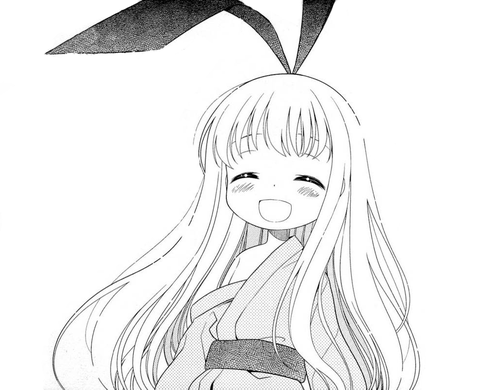
\includegraphics[width=0.5\textwidth]{image/166.png}
\vfill

\newpage
\section*{\underline{信息科学与工程}学院课程设计成绩评价表}
\addcontentsline{toc}{section}{成绩评价表}
\CTEXnoindent
课程名称:数据结构课程设计\\
设计题目:探究压缩算法\\
专业:计算机\hfill 班级:1303 班\hfill 姓名:田劲锋\hfill 学号:201316920311\\[0.5em]
\begin{tabularx}{\textwidth}[c]{|c|c|c|X|}\hline
序号 & 评审项目 & 分\quad 数 & \multicolumn{1}{c|}{满分标准说明} \\\hline
1 & 内容 &  & 思路清晰;语言表达准确,概念清楚,论点正确;实验方法科学,分析归纳合理;结论严谨,设计有应用价值。任务饱满,做了大量的工作。 \\\hline
2 & 创新 &  &  内容新颖,题目能反映新技术,对前人工作有改进或突破,或有独特见解 \\\hline
3 & \tabincell{c}{完整性\\实用性} & & 整体构思合理,理论依据充分,设计完整,实用性强 \\\hline
4 & \tabincell{c}{数据准确\\可靠} & & 数据准确,公式推导正确 \\\hline
5 & 规范性 &  & 设计格式、绘图、图纸、实验数据、标准的运用等符合有关标准和规定 \\\hline
6 & 纪律性 &  & 能很好的遵守各项纪律,设计过程认真; \\\hline
7 & 答辩 &  & 准备工作充分,回答问题有理论依据,基本概念清楚。主要问题回答简明准确。在规定的时间内作完报告。 \\\hline
\tabincell{c}{总\\分} & \multicolumn{3}{c|}{} \\\hline
\tabincell{c}{综\\合\\意\\见} & \multicolumn{3}{r|}{\tabincell{r}{\vspace*{4cm}\\
\qquad 指导教师:\hspace*{8em} \qquad 年\quad 月\quad 日\quad\\[1em]
}} \\\hline
\end{tabularx}
\CTEXindent

%%%% 结束 %%%%

\end{document}
